%%%%%%%%%%%%%%%%%%%%%%%%%%%%%%%%%%%%%%%%%%%%%%%%%%%%%%%%%%%%%%%%%%%%%%%%%%
%%LaTeX template for papers && theses									%%
%%Done by the incredible ||Z01db3rg||									%%
%%Under the do what ever you want license								%%
%%%%%%%%%%%%%%%%%%%%%%%%%%%%%%%%%%%%%%%%%%%%%%%%%%%%%%%%%%%%%%%%%%%%%%%%%% 

%start preamble
\documentclass[paper=a4,fontsize=11pt]{scrartcl}%kind of doc, font size, paper size
\usepackage[ngerman]{babel}%for special german letters etc			
%\usepackage{t1enc} obsolete, but some day we go back in time and could use this again
\usepackage[T1]{fontenc}%same as t1enc but better						
\usepackage[utf8]{inputenc}%utf-8 encoding, other systems could use others encoding
%\usepackage[latin9]{inputenc}			
\usepackage{amsmath}%get math done
\usepackage{amsthm}%get theorems and proofs done
\usepackage{graphicx}%get pictures & graphics done
\graphicspath{{pictures/}}%folder to stash all kind of pictures etc
\usepackage[pdftex,hidelinks]{hyperref}%for links to web
\usepackage{amssymb}%symbolics for math
\usepackage{amsfonts}%extra fonts
\usepackage []{natbib}%citation style
\usepackage{caption}%captions under everything
\usepackage{listings}
\usepackage[titletoc]{appendix}
\numberwithin{equation}{section} 
\usepackage[printonlyused,withpage]{acronym}%how to handle acronyms
\usepackage{float}%for garphics and how to let them floating around in the doc
\usepackage{cclicenses}%license!
\usepackage{xcolor}%nicer colors, here used for links
\usepackage{wrapfig}%making graphics floated by text and not done by minipage
\usepackage{dsfont}
\usepackage{stmaryrd}
\usepackage{geometry}
\usepackage{hyperref}
\usepackage{fancyhdr}
\usepackage{menukeys}

\pagestyle{fancy}
\lhead{Benjamin Tröster\\Netzwerke Übung}
\rhead{FB 4 -- Angewandte Informatik\\ HTW-Berlin}
\lfoot{Virtualisierung mit VirtualBox}
\cfoot{}
\fancyfoot[R]{\thepage}
\renewcommand{\headrulewidth}{0.4pt}
\renewcommand{\footrulewidth}{0.4pt}

\lstdefinestyle{Bash}{
  language=bash,
  showstringspaces=false,
  basicstyle=\small\sffamily,
  numbers=left,
  numberstyle=\tiny,
  numbersep=5pt,
  frame=trlb,
  columns=fullflexible,
  backgroundcolor=\color{gray!20},
  linewidth=0.9\linewidth,
  %xleftmargin=0.5\linewidth
}

\newlength\labelwd
\settowidth\labelwd{\bfseries viii.)}
\usepackage{tasks}
\settasks{counter-format =tsk[a].), label-format=\bfseries, label-offset=3em, label-align=right, label-width
=\labelwd, before-skip =\smallskipamount, after-item-skip=0pt}
\usepackage[inline]{enumitem}
\setlist[enumerate]{% (
labelindent = 0pt, leftmargin=*, itemsep=12pt, label={\textbf{\arabic*.)}}}

\pdfpkresolution=2400%higher resolution

%%here begins the actual document%%
\newcommand{\horrule}[1]{\rule{\linewidth}{#1}} % Create horizontal rule command with 1 argument of height

\DeclareMathOperator{\id}{id}

\begin{document}
\begin{center}
\Large{\textbf{Nutzung von Virtualisierung -- VirtualBox}}
\end{center}
\begin{center}\Large{\textbf{Virtualisierungssoftware}}\end{center}\vskip0.25in
Virtualisierungssoftware sind Programmpakete, welche es ermöglichen auf einem physischen Rechner weitere logische Rechner in Software zu simulieren. In diesen Virtuellen Maschinen kann ein Betriebssystem wie auf einem physischen Rechner, mit beliebiger Software (sofern von der Emulation erlaubt) betrieben werden.\\
Eine kurze Auswahl von Virtualisierungsumgebungen:
\begin{itemize}
	\item VMWare: \url{http://www.vmware.com} -- Multi-Plattform
	\item XEN: \url{http://www.xenproject.org} -- Linux
	\item Oracle VirtualBox: \url{http://www.virtualbox.org} -- Multi-Plattform
	\item Parallels Desktop: \url{http://www.parallels.com} -- OSx
\end{itemize}

\begin{center}
\Large{\textbf{Virtuelle Maschinen}}
\end{center}
Eine Virtuelle Maschine (VM) besteht bei allen Systemen (VirtualBox, VMWare, ...) aus einer Konfigurationsdatei, in der die simulierte Hardware festgelegt wird und einer/ mehrerer großer Dateien, die als Massenspeicher für die VM dienen. Zum Verschieben einer virtuellen Maschine auf einen anderen Rechner müssen sie einfach das Verzeichnis mit diesen Dateien kopieren.\\
Wenn nach dem Start der VM ein Dialogfenster mit der Frage kommt, ob Sie diese VM verschoben oder kopiert haben, sollten Sie im Labor kopiert antworten. Grund hierfür sind die von der VM genutzten MAC-Adressen -- bei verschoben VMs bleiben die MAC-Adressen gleich, bei kopierten generiert VirtualBox automatisch neue, zufällige MAC-Adressen. Somit ist sicher gestellt, dass es keine doppelten MAC-Adressen im Pool gibt, da alle VMs auf allen Rechnern nur Kopien einer VM sind.\\
Sollte es beim Import einer VM (VirtualBox Manager Program -- Menü: Machine -- Hinzufügen) eine Fehlermeldung geben, dass die Konfigurationsdatei nicht gültig sei, so öffnen Sie diese bitte in einem
Texteditor (die *.vbox Datei im Verzeichnis) und prüfen Sie die XML-Syntax. Es kam beim Kopieren und automatischen Anpassen der Datei manchmal vor, das ein schließende spitze Klammer am Ende nicht richtig gesetzt wurde.
\begin{center}
\Large{\textbf{Netzwerkeinstellungen der VMs}}
\end{center}
In VirtualBox legen Sie in den Netzwerkeinstellungen jeder VM fest, mit welches der Netze die
Netzwerkpaketes des VM-Gastes weitergeleitet werden. Diese Einstellung können Sie auch beliebig zur
Laufzeit ändern -- ein Neustart der VM ist dazu nicht notwendig.\\
\begin{figure}[H]
	\centering
	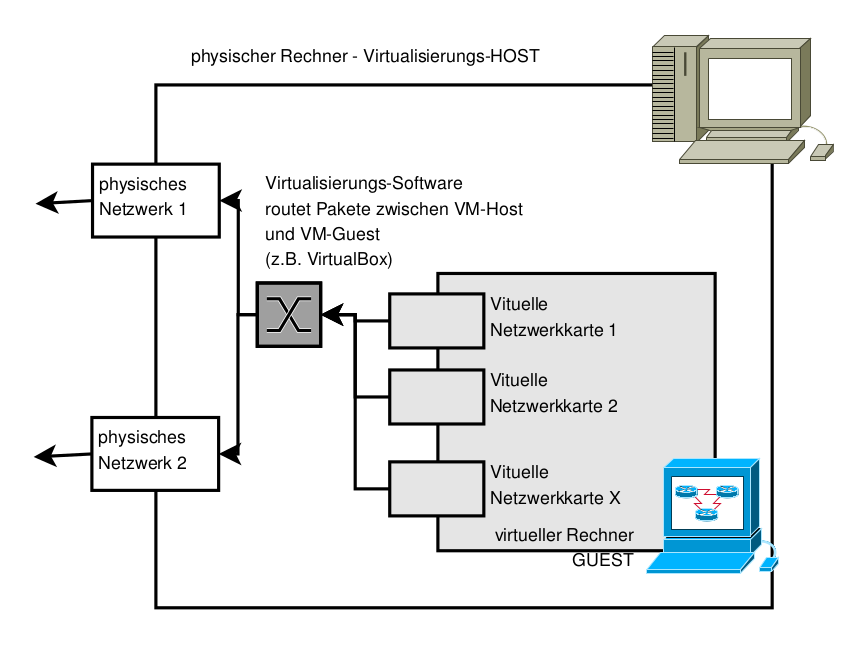
\includegraphics[scale=0.4]{vbox1}
	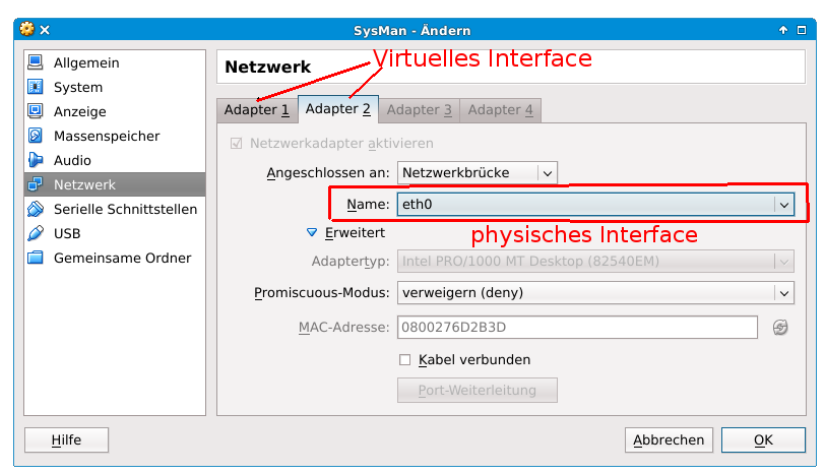
\includegraphics[scale=0.4]{vbox2}
\end{figure}
Im laufenden Betrieb der VM können Sie im Fenstermodus unten links mittels des Icons mit den zwei
kleinen Monitoren nachschauen, wie die Netzwerkkarten aktuell konfiguriert sind. Dazu warten Sie mit
der Maus entweder ein paar Sekunden über dem Icon bis ein kleines Infofenster erscheint (Abbildung
\ref{vbox3}) oder, wenn Sie mit der rechten Maustaste auf dieses Icon klicken, erhalten Sie einen Dialog, mit dem Sie die Einstellungen im laufenden Betrieb umstellen können (s. Abb. \ref{vbox4}).
\begin{figure}[H]
\centering
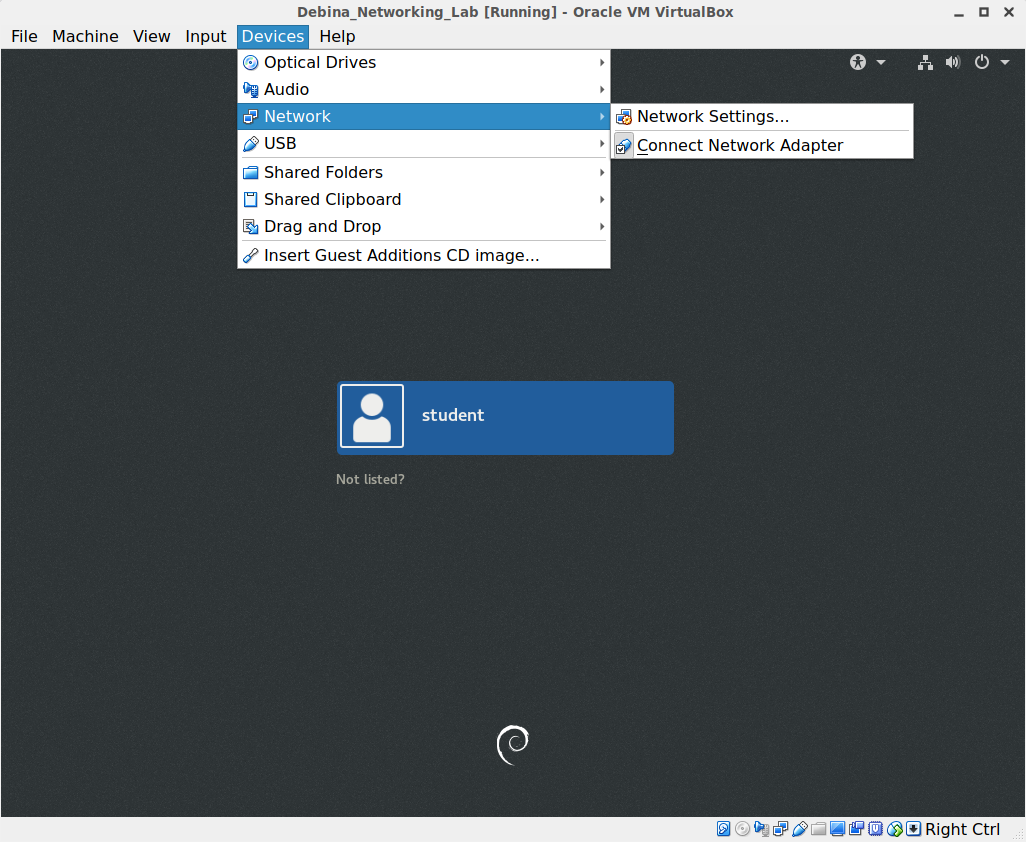
\includegraphics[scale=0.4]{vbox3}
\caption{Zugriff auf Netzwerkeinstellungen via Menüleiste}
\label{vbox3}
\end{figure}
\begin{figure}[H]
\centering
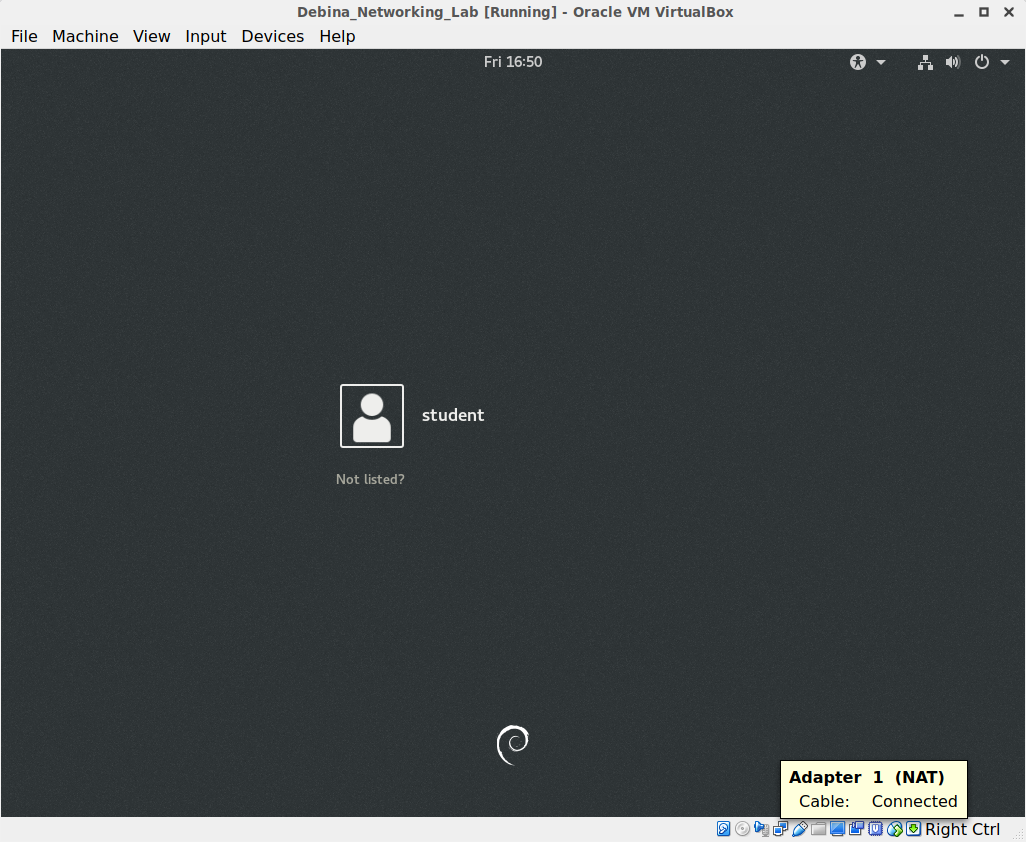
\includegraphics[scale=0.4]{vbox4}
\caption{Zugriff auf Netzwerkeinstellungen via Icons am unteren Rand}
\label{vbox4}
\end{figure}
Bei den Netzwerkkarten können Sie mehrere verschiedene Modi einstellen -- für Sie interessant
sind aber nur zwei: NAT und Bridge. Die anderen Formen können Sie bei Bedarf in der Dokumentation von VirtualBox nachlesen (\url{https://www.virtualbox.org/manual/ch06.html}).
\begin{center}
\Large{\textbf{Netzwerkmodus: NAT}}
\end{center}
Im Modus NAT werden alle Netzwerkpakete bevor sie von VirtualBox von der VM zum physischen Rechner weitergeleitet werden, umgeschrieben. Damit ist es möglich, dass nach außen die gleiche IP-Adresse Ihres Routers genutzt werden kann. Dies wird in den meisten Fällen unter IPv4 ohnehin getan.
\begin{figure}[H]
\centering
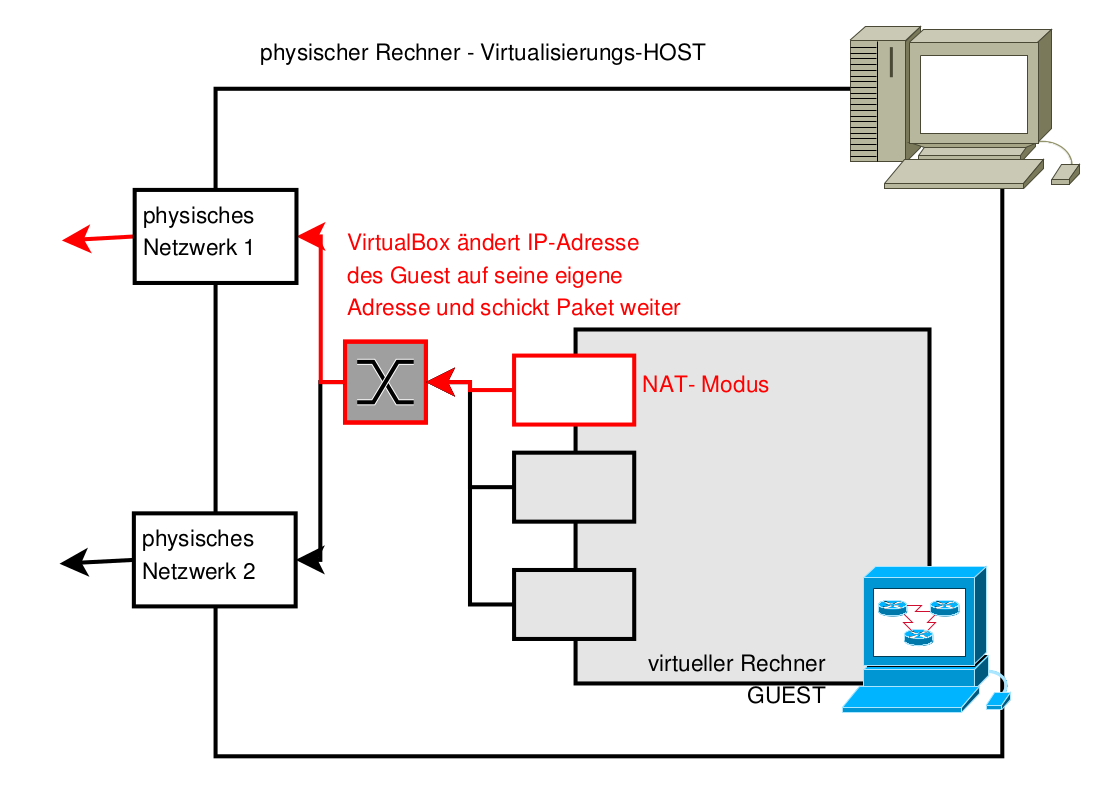
\includegraphics[scale=0.35]{vbox5}
\caption{Virtualisierte Netzwerkkarte im NAT-Modus}
\end{figure}
\begin{center}
\Large{\textbf{Netzwerkmodus: Bridge}}
\end{center}
Im Modus Bridge werden alle von der VM erzeugten Pakete sofort ohne eine Änderung durch VirtualBox an die physische Netzwerkkarte weitergereicht und über das Kabel versendet. Dabei muss in den Netzwerkeinstellungen von VirtualBox festgelegt werden, auf welche der Netzwerkkarten des physischen Rechners die Pakete weitergeleitet werden -- somit werden Pakete nur an diese eine Netzwerkkarte gesendet. Das genutzte Interface legen Sie in den Einstellungen für jedes virtuelle Interface getrennt fest. Zur Laufzeit können Sie die Zuordnung auch nachträglich noch ändern. In diesem Modus sieht es für andere Rechner so aus, als ob zwei vollkommen eigenständige Rechner im Netzwerk aktiv sind. Zum einen der physische Host und zum anderen die VM. Damit können sich auch alle VMs untereinander direkt per Netzwerk erreichen.
\begin{figure}[H]
\centering
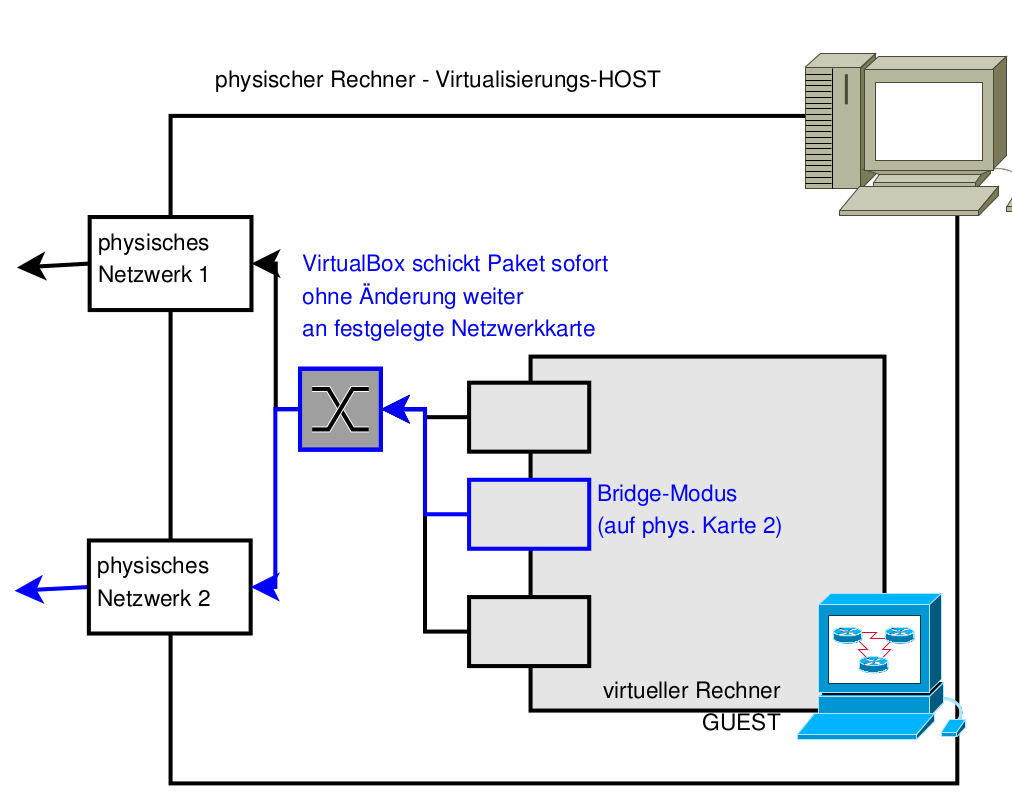
\includegraphics[scale=0.35]{vbox6}
\caption{Virtualisierte Netzwerkkarte im Bridge-Modus}
\end{figure}
\end{document}